% F087｜牛顿切线法快速求近似根
% 保留上传模板中的 \Conclusion 与 01_function 引用层级；若项目实际模块目录不同，按真实目录调整前缀。
\Conclusion
\subsection{F087 牛顿切线法快速求近似根}
% F087｜牛顿切线法快速求近似根｜01_statement.tex
% 继承上传模板的 LaTeX 环境；当前条目的内容独立编写。
\clearpage
\begin{statementbox}
\textbf{\textcolor{CStatement}{为什么用切线找根}}
\par\medskip
\begin{center}
% F087｜tangent 原创简明教学示意图
\begin{tikzpicture}[>=stealth,scale=.82]
\draw[->] (0,0)--(7.6,0) node[right]{$x$};\draw[->] (.8,-1.4)--(.8,3.2) node[above]{$y$};
% 横向比例尺 x_point=8(x-2.65)，纵向比例尺 y_point=0.75(x^2-10)。
\draw[teal,thick,domain=2.76:3.48,samples=45] plot ({8*(\x-2.65)},{.75*(\x*\x-10)});
% 在真实点 x_0=3 的切线；交轴位置 x_1=19/6。
\draw[orange,thick] (2,-1.2)--(6,1.05);
\fill[orange] (2.8,-.75) circle (2pt) node[below left=5pt]{$x_0=3$};
\fill[orange] (4.1333,0) circle(2pt) node[below=7pt]{$x_1\approx3.1667$};
\node at (5.5,2.7){\small 用切线寻找新的交点};
\node[teal] at (5.7,1.9){\small $y=x^2-10$};
\end{tikzpicture}

\end{center}
\medskip
方程 $x^2-10=0$ 的正根在 $3$ 与 $4$ 之间。把曲线在 $x=3$ 附近用一小段切线代替，切线与横轴的交点就给出新的猜测值。重复做，通常能越来越接近真正的根。
\end{statementbox}
\clearpage
\begin{statementbox}
\textbf{\textcolor{CStatement}{三个最有用的公式}}
\par\medskip
\begin{center}
% F087｜square 原创简明教学示意图
\begin{tikzpicture}[>=stealth,scale=.9]
\node[draw,fill=teal!8,rounded corners,minimum width=7.3cm,minimum height=1.5cm,align=center] at (4,0) {$x_{n+1}=\dfrac12\left(x_n+\dfrac{A}{x_n}\right)$};
\node at (4,-1.2) {\small 正数 $x_n$ 与 $A/x_n$ 的平均数};
\end{tikzpicture}

\end{center}
\medskip
\[x_{n+1}=x_n-\frac{f(x_n)}{f'(x_n)}.\]求平方根：$x_{n+1}=\dfrac12(x_n+A/x_n)$；求正数的立方根：$x_{n+1}=\dfrac{2x_n+A/x_n^2}{3}$。后两个只是第一个公式的具体应用。
\end{statementbox}

% F087｜牛顿切线法快速求近似根｜02_explanation.tex
% 继承上传模板的 LaTeX 环境；当前条目的内容独立编写。
\clearpage
\begin{explanationbox}
\textbf{\textcolor{CExplanation}{看图理解：为什么出现减法}}
\par\medskip
\begin{center}
% F087｜tangent 原创简明教学示意图
\begin{tikzpicture}[>=stealth,scale=.82]
\draw[->] (0,0)--(7.6,0) node[right]{$x$};\draw[->] (.8,-1.4)--(.8,3.2) node[above]{$y$};
% 横向比例尺 x_point=8(x-2.65)，纵向比例尺 y_point=0.75(x^2-10)。
\draw[teal,thick,domain=2.76:3.48,samples=45] plot ({8*(\x-2.65)},{.75*(\x*\x-10)});
% 在真实点 x_0=3 的切线；交轴位置 x_1=19/6。
\draw[orange,thick] (2,-1.2)--(6,1.05);
\fill[orange] (2.8,-.75) circle (2pt) node[below left=5pt]{$x_0=3$};
\fill[orange] (4.1333,0) circle(2pt) node[below=7pt]{$x_1\approx3.1667$};
\node at (5.5,2.7){\small 用切线寻找新的交点};
\node[teal] at (5.7,1.9){\small $y=x^2-10$};
\end{tikzpicture}

\end{center}
\medskip
在 $(x_n,f(x_n))$ 点作切线。若切线斜率为 $k$，向横轴移动时纵坐标要从 $f(x_n)$ 变为 $0$，横向需要移动 $-f(x_n)/k$，因此新横坐标是 $x_n-f(x_n)/k$。
\end{explanationbox}
\clearpage
\begin{explanationbox}
\textbf{\textcolor{CExplanation}{平方根为什么是“取平均”}}
\par\medskip
\begin{center}
% F087｜square 原创简明教学示意图
\begin{tikzpicture}[>=stealth,scale=.9]
\node[draw,fill=teal!8,rounded corners,minimum width=7.3cm,minimum height=1.5cm,align=center] at (4,0) {$x_{n+1}=\dfrac12\left(x_n+\dfrac{A}{x_n}\right)$};
\node at (4,-1.2) {\small 正数 $x_n$ 与 $A/x_n$ 的平均数};
\end{tikzpicture}

\end{center}
\medskip
用 $f(x)=x^2-A$，切线斜率 $f'(x)=2x$。\[x_{n+1}=x_n-\frac{x_n^2-A}{2x_n}=\frac12\left(x_n+\frac A{x_n}\right).\]如果猜得偏大，$A/x_n$ 会偏小；取两者平均就能调整。
\end{explanationbox}
\clearpage
\begin{explanationbox}
\textbf{\textcolor{CExplanation}{什么时候不该盲用}}
\par\medskip
\begin{center}
% F087｜steps 原创简明教学示意图
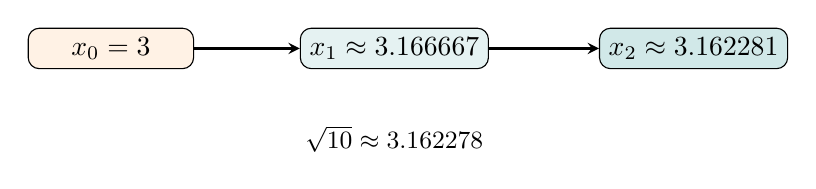
\begin{tikzpicture}[>=stealth,node distance=1cm]
\node[draw,rounded corners,fill=orange!10,minimum width=2.1cm] (a) at (0,0) {$x_0=3$};
\node[draw,rounded corners,fill=teal!10,minimum width=2.3cm] (b) at (3.6,0) {$x_1\approx3.166667$};
\node[draw,rounded corners,fill=teal!18,minimum width=2.3cm] (c) at (7.4,0) {$x_2\approx3.162281$};
\draw[->,thick] (a)--(b);\draw[->,thick] (b)--(c);
\node at (3.6,-1.15) {\small $\sqrt{10}\approx3.162278$};
\end{tikzpicture}

\end{center}
\medskip
切线可能几乎水平，也可能把新点推向很远处。只有在函数足够平滑、初值选得合适时，连续更新才会有效。对一个具体问题，算完应将结果代回原方程检验。
\end{explanationbox}

% F087｜牛顿切线法快速求近似根｜03_proof.tex
% 继承上传模板的 LaTeX 环境；当前条目的内容独立编写。
\clearpage
\begin{proofbox}
\textbf{\textcolor{CProof}{证明一（门槛最低）：从切线方程推导}}
\par\medskip
\begin{center}
% F087｜tangent 原创简明教学示意图
\begin{tikzpicture}[>=stealth,scale=.82]
\draw[->] (0,0)--(7.6,0) node[right]{$x$};\draw[->] (.8,-1.4)--(.8,3.2) node[above]{$y$};
% 横向比例尺 x_point=8(x-2.65)，纵向比例尺 y_point=0.75(x^2-10)。
\draw[teal,thick,domain=2.76:3.48,samples=45] plot ({8*(\x-2.65)},{.75*(\x*\x-10)});
% 在真实点 x_0=3 的切线；交轴位置 x_1=19/6。
\draw[orange,thick] (2,-1.2)--(6,1.05);
\fill[orange] (2.8,-.75) circle (2pt) node[below left=5pt]{$x_0=3$};
\fill[orange] (4.1333,0) circle(2pt) node[below=7pt]{$x_1\approx3.1667$};
\node at (5.5,2.7){\small 用切线寻找新的交点};
\node[teal] at (5.7,1.9){\small $y=x^2-10$};
\end{tikzpicture}

\end{center}
\medskip
切线方程为 $y-f(x_n)=f'(x_n)(x-x_n)$。令 $y=0$，则 $-f(x_n)=f'(x_n)(x_{n+1}-x_n)$，所以\[\boxed{x_{n+1}=x_n-\frac{f(x_n)}{f'(x_n)}}.\]这里必须要求 $f'(x_n)\ne0$。
\end{proofbox}
\clearpage
\begin{proofbox}
\textbf{\textcolor{CProof}{证明二（最快）：平方根的代数推导}}
\par\medskip
\begin{center}
% F087｜square 原创简明教学示意图
\begin{tikzpicture}[>=stealth,scale=.9]
\node[draw,fill=teal!8,rounded corners,minimum width=7.3cm,minimum height=1.5cm,align=center] at (4,0) {$x_{n+1}=\dfrac12\left(x_n+\dfrac{A}{x_n}\right)$};
\node at (4,-1.2) {\small 正数 $x_n$ 与 $A/x_n$ 的平均数};
\end{tikzpicture}

\end{center}
\medskip
设 $A>0,x_n>0$，将 $f(x)=x^2-A$、$f'(x)=2x$ 代入切线式，整理即得\[x_{n+1}=\frac{x_n^2+A}{2x_n}=\frac12\left(x_n+\frac A{x_n}\right).\]若 $r=\sqrt A$，还可验证 $x_{n+1}-r=\dfrac{(x_n-r)^2}{2x_n}\ge0$。
\end{proofbox}
\clearpage
\begin{proofbox}
\textbf{\textcolor{CProof}{证明三（迁移到立方根）：直接换函数}}
\par\medskip
\begin{center}
% F087｜cube 原创简明教学示意图
\begin{tikzpicture}[>=stealth,scale=.88]
\node[draw,rounded corners,fill=teal!8,minimum width=8cm,minimum height=1.3cm] (a) at (4,0) {$x_{n+1}=\dfrac{2x_n+A/x_n^2}{3}$};
\node at (4,-1.0) {\small 三次根号也能用切线修正，不必背另一套思路};
\end{tikzpicture}

\end{center}
\medskip
设 $A>0,x_n>0$。令 $f(x)=x^3-A$，则 $f'(x)=3x^2$，因此\[x_{n+1}=x_n-\frac{x_n^3-A}{3x_n^2}=\frac{2x_n+A/x_n^2}{3}.\]方法并未变化：\textbf{先写方程，再求切线，最后求横轴交点。}
\end{proofbox}

% F087｜牛顿切线法快速求近似根｜04_examples.tex
% 继承上传模板的 LaTeX 环境；当前条目的内容独立编写。
\clearpage
\begin{examplebox}
\textbf{\textcolor{CExample}{例 1：两次逼近根号 10}}
\par\medskip
\begin{center}
% F087｜steps 原创简明教学示意图
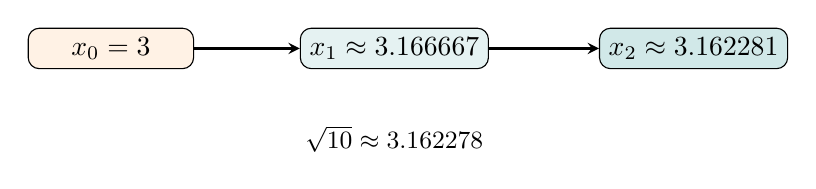
\begin{tikzpicture}[>=stealth,node distance=1cm]
\node[draw,rounded corners,fill=orange!10,minimum width=2.1cm] (a) at (0,0) {$x_0=3$};
\node[draw,rounded corners,fill=teal!10,minimum width=2.3cm] (b) at (3.6,0) {$x_1\approx3.166667$};
\node[draw,rounded corners,fill=teal!18,minimum width=2.3cm] (c) at (7.4,0) {$x_2\approx3.162281$};
\draw[->,thick] (a)--(b);\draw[->,thick] (b)--(c);
\node at (3.6,-1.15) {\small $\sqrt{10}\approx3.162278$};
\end{tikzpicture}

\end{center}
\medskip
取 $x_0=3$，\[x_1=\frac12\left(3+\frac{10}{3}\right)=\frac{19}{6}\approx3.166667.\]再算 $x_2=\dfrac12\left(\frac{19}{6}+\frac{60}{19}\right)=\frac{721}{228}\approx3.162281$；而 $\sqrt{10}\approx3.162278$。两步已很接近。
\end{examplebox}
\clearpage
\begin{examplebox}
\textbf{\textcolor{CExample}{例 2：估算立方根 71}}
\par\medskip
\begin{center}
% F087｜cube 原创简明教学示意图
\begin{tikzpicture}[>=stealth,scale=.88]
\node[draw,rounded corners,fill=teal!8,minimum width=8cm,minimum height=1.3cm] (a) at (4,0) {$x_{n+1}=\dfrac{2x_n+A/x_n^2}{3}$};
\node at (4,-1.0) {\small 三次根号也能用切线修正，不必背另一套思路};
\end{tikzpicture}

\end{center}
\medskip
$4^3=64<71<125=5^3$，取 $x_0=4$：\[x_1=\frac{2\cdot4+71/4^2}{3}=\frac{199}{48}\approx4.145833.\]代回立方后可知仍略偏大，再迭代一次约为 $4.140824$；真值约 $4.140818$。
\end{examplebox}
\clearpage
\begin{examplebox}
\textbf{\textcolor{CExample}{例 3：只比较大小，不需要迭代}}
\par\medskip
\begin{center}
% F087｜tangent 原创简明教学示意图
\begin{tikzpicture}[>=stealth,scale=.82]
\draw[->] (0,0)--(7.6,0) node[right]{$x$};\draw[->] (.8,-1.4)--(.8,3.2) node[above]{$y$};
% 横向比例尺 x_point=8(x-2.65)，纵向比例尺 y_point=0.75(x^2-10)。
\draw[teal,thick,domain=2.76:3.48,samples=45] plot ({8*(\x-2.65)},{.75*(\x*\x-10)});
% 在真实点 x_0=3 的切线；交轴位置 x_1=19/6。
\draw[orange,thick] (2,-1.2)--(6,1.05);
\fill[orange] (2.8,-.75) circle (2pt) node[below left=5pt]{$x_0=3$};
\fill[orange] (4.1333,0) circle(2pt) node[below=7pt]{$x_1\approx3.1667$};
\node at (5.5,2.7){\small 用切线寻找新的交点};
\node[teal] at (5.7,1.9){\small $y=x^2-10$};
\end{tikzpicture}

\end{center}
\medskip
判断 $\sqrt{10}>3.16$ 吗？直接验算 $3.16^2=9.9856<10$ 即可。\textbf{切线法适合求近似数值，不必每题都用。}
\end{examplebox}

% F087｜牛顿切线法快速求近似根｜05_traps.tex
% 继承上传模板的 LaTeX 环境；当前条目的内容独立编写。
\clearpage
\begin{trapbox}
\textbf{\textcolor{CTrap}{易错一：把零点误认为函数最低点}}
\par\medskip
\begin{center}
% F087｜tangent 原创简明教学示意图
\begin{tikzpicture}[>=stealth,scale=.82]
\draw[->] (0,0)--(7.6,0) node[right]{$x$};\draw[->] (.8,-1.4)--(.8,3.2) node[above]{$y$};
% 横向比例尺 x_point=8(x-2.65)，纵向比例尺 y_point=0.75(x^2-10)。
\draw[teal,thick,domain=2.76:3.48,samples=45] plot ({8*(\x-2.65)},{.75*(\x*\x-10)});
% 在真实点 x_0=3 的切线；交轴位置 x_1=19/6。
\draw[orange,thick] (2,-1.2)--(6,1.05);
\fill[orange] (2.8,-.75) circle (2pt) node[below left=5pt]{$x_0=3$};
\fill[orange] (4.1333,0) circle(2pt) node[below=7pt]{$x_1\approx3.1667$};
\node at (5.5,2.7){\small 用切线寻找新的交点};
\node[teal] at (5.7,1.9){\small $y=x^2-10$};
\end{tikzpicture}

\end{center}
\medskip
牛顿切线法一般寻找的是\textbf{$f(x)=0$ 的根}，不是自动寻找最低点。对 $f(x)=x^2-10$，正根是图像与横轴的交点，最低点却在 $x=0$。
\end{trapbox}
\clearpage
\begin{trapbox}
\textbf{\textcolor{CTrap}{易错二：忘记斜率不能为零}}
\par\medskip
\begin{center}
% F087｜square 原创简明教学示意图
\begin{tikzpicture}[>=stealth,scale=.9]
\node[draw,fill=teal!8,rounded corners,minimum width=7.3cm,minimum height=1.5cm,align=center] at (4,0) {$x_{n+1}=\dfrac12\left(x_n+\dfrac{A}{x_n}\right)$};
\node at (4,-1.2) {\small 正数 $x_n$ 与 $A/x_n$ 的平均数};
\end{tikzpicture}

\end{center}
\medskip
分母是 $f'(x_n)$，若为 $0$，公式不能直接使用。如对 $x^2-10$ 取 $x_0=0$，则除数为零；求正平方根应取正的初值。
\end{trapbox}
\clearpage
\begin{trapbox}
\textbf{\textcolor{CTrap}{易错三：把“迭代几次很准”理解为永远收敛}}
\par\medskip
\begin{center}
% F087｜steps 原创简明教学示意图
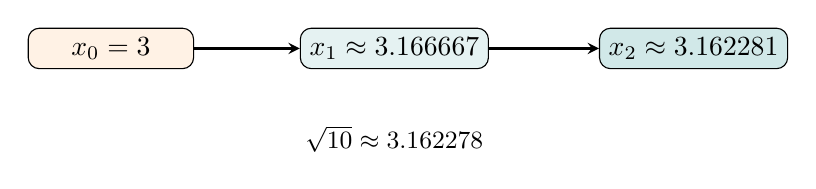
\begin{tikzpicture}[>=stealth,node distance=1cm]
\node[draw,rounded corners,fill=orange!10,minimum width=2.1cm] (a) at (0,0) {$x_0=3$};
\node[draw,rounded corners,fill=teal!10,minimum width=2.3cm] (b) at (3.6,0) {$x_1\approx3.166667$};
\node[draw,rounded corners,fill=teal!18,minimum width=2.3cm] (c) at (7.4,0) {$x_2\approx3.162281$};
\draw[->,thick] (a)--(b);\draw[->,thick] (b)--(c);
\node at (3.6,-1.15) {\small $\sqrt{10}\approx3.162278$};
\end{tikzpicture}

\end{center}
\medskip
任意方程或任意起点都可能失败；尤其初值离根太远、切线接近平行横轴时。算完必须代回检验。
\end{trapbox}

% F087｜牛顿切线法快速求近似根｜06_summary.tex
% 继承上传模板的 LaTeX 环境；当前条目的内容独立编写。
\clearpage
\begin{summarybox}
\textbf{\textcolor{CSummary}{快记、快懂、快用}}
\par\medskip
\begin{center}
% F087｜steps 原创简明教学示意图
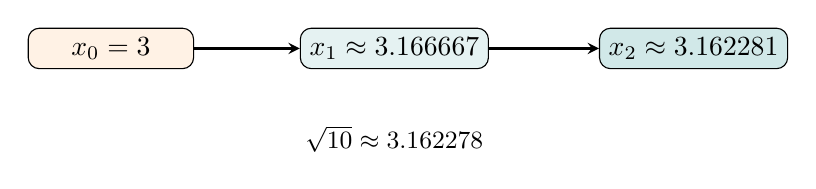
\begin{tikzpicture}[>=stealth,node distance=1cm]
\node[draw,rounded corners,fill=orange!10,minimum width=2.1cm] (a) at (0,0) {$x_0=3$};
\node[draw,rounded corners,fill=teal!10,minimum width=2.3cm] (b) at (3.6,0) {$x_1\approx3.166667$};
\node[draw,rounded corners,fill=teal!18,minimum width=2.3cm] (c) at (7.4,0) {$x_2\approx3.162281$};
\draw[->,thick] (a)--(b);\draw[->,thick] (b)--(c);
\node at (3.6,-1.15) {\small $\sqrt{10}\approx3.162278$};
\end{tikzpicture}

\end{center}
\medskip
\textbf{快记：}新点 $=$ 旧点 $-$“函数值 $\div$ 斜率”。\par\textbf{快懂：}用局部切线代替曲线，从切线横轴交点更新。\par\textbf{快用：}根号的迭代公式计算简便；只比较大小时优先直接平方。
\end{summarybox}
\clearpage
\begin{summarybox}
\textbf{\textcolor{CSummary}{和平方根估算的联系}}
\par\medskip
\begin{center}
% F087｜square 原创简明教学示意图
\begin{tikzpicture}[>=stealth,scale=.9]
\node[draw,fill=teal!8,rounded corners,minimum width=7.3cm,minimum height=1.5cm,align=center] at (4,0) {$x_{n+1}=\dfrac12\left(x_n+\dfrac{A}{x_n}\right)$};
\node at (4,-1.2) {\small 正数 $x_n$ 与 $A/x_n$ 的平均数};
\end{tikzpicture}

\end{center}
\medskip
F086 的近似 $t+(A-t^2)/(2t)$，正好就是 F087 对 $x^2-A=0$ 从 $x_0=t$ 出发的\textbf{第一次迭代}。两条结论角度不同：F086 主讲估值与误差，F087 主讲切线与重复更新。
\end{summarybox}

